Un sistema USB posee un esquema %de bus maestro-esclavo 
en forma de árbol cuyo nodo principal es el host. Es decir, la comunicación se realiza siempre a través de una única línea a la que se conectan todos los dispositivos (bus). Dado el campo de direcciones provisto por la norma, un sistema USB puede conectar hasta 128 dispositivos. El acceso al bus es administrado por un maestro. El maestro se encarga de solicitar a cada uno de los dispositivos su intervención. Posteriormente, el dispositivo debe responder al pedido del maestro. Este esquema es lo que se conoce como maestro-esclavo. De esta forma, el sistema se asegura que el bus sea utilizado por un dispositivo a la vez para enviar o recibir datos.\\

En un sistema USB no cualquier dispositivo puede ser maestro. Este rol lo cumple solo uno: una PC, o cualquier dispositivo con capacidad de llevar a cabo las tareas asignadas (que se detallan más adelante); denominado Host por la norma. La palabra {\it HOST} proviene del habla inglesa y se traduce como anfitrión, aunque en la jerga se conoce comunmente por su nombre en inglés.\\

\begin{figure}[]
	\centering
	\begin{tikzpicture}[scale=.87,>=latex,level 1/.append style={level distance = 2ex},level 2/.append style={level distance = 40}]
		\begin{scope}
			\begin{scope}[transform shape,grow = down]
				\node[] (host) {\it HOST} [
				sibling distance=60,
%				growth parent anchor=south, 
%				edge from parent fork down,
				]
				child{node[](l1r){Raíz}edge from parent[draw=none]
					child{node[](l2h1){Hub}
						child{node[](l3f1){Función}
						}
						child{node[](l3h1){Hub}
							child{node[](l4h1){Hub}
								child{node[](l5h1){Hub}
									child{node[](l6f1){Función}
									}
									child{node[](l6h1){Hub}
										child{node[](l7f1){Función}
										}
									}
								}
								child{node[](l5f1){Función}
								}
							}
						}
						child{node[] (l3f2) {Función}}
					}
					child{node[](l2f1){Función}}
					child{node[](l2h2){Hub}
						child{node[](l3h2){Hub}
							child{node[](l4f1){Función}
							}
							child{node[](l4f2){Función}
							}
						}
					}
				};
				\node[](l6)[left=of l6f1]{Grada 6};
				\node[](l7)at(l6|-l7f1){Grada 7};
				\node[](l5)at(l6|-l5h1){Grada 5};
				\node[](l4)at(l5|-l4h1){Grada 4};
				\node[](l3)at(l4|-l3f1){Grada 3};
				\node[](l2)at(l3|-l2h1){Grada 2};
				\node[](l1)at(l2|-l1r){Grada 1};
			\end{scope}
			\begin{scope}[dashed]
				\draw (l7) -| (l7f1.west);
				\draw (l6) -| (l6f1.west);
%					\draw(l6f1)--(l6h1);
				\draw (l5) -| (l5h1.west);
%					\draw(l5h1)--(l5h1);
				\draw (l4) -| (l4h1.west);
%					\draw(l4h1)--(l4f1);
%					\draw(l4f1)--(l4f2);
				\draw (l3) -| (l3f1.west);
%					\draw(l3f1)--(l3h1);
%					\draw(l3h1)--(l3f2);
%					\draw(l3f2)--(l3h2);
				\draw (l2) -| (l2h1.west);
%					\draw(l2h1)--(l2f1);
%					\draw(l2f1)--(l2h2);
				\draw (l1) -| (l1r.west);
			\end{scope}
		\end{scope}
	\end{tikzpicture}	
	\caption{Topología de un sistema USB}
	\label{fig:top}
\end{figure}

La topología del bus, la que se observa en la Figura \ref{fig:top}, posee forma de árbol, es decir, puede ser pensada como una comunicación vertical, donde en el punto más alto se encuentra el Host. Siguiendo hacia abajo, el bus puede encontrar dos tipos diferentes de dispositivos: Funciones, cuyo rol es el de proveer una utilidad al sistema, como ser la de captura de imagen, reproducción de audio o el ingreso de comandos; y Hubs (concentradores o distribuidores), que se encargan de conectar una o más funciones al sistema. La norma USB establece gradas, en donde cada Hub introduce una nueva grada que contiene a las Funciones conectadas. Por cuestiones de restricciones temporales y tiempos de propagación en los cables, no se permiten más de 7 gradas, incluyendo al Host en la primera. Es decir, no se puede conectar más de 5 Hubs en cascada. La grada 7 sólo puede contener Funciones\cite{USBspec}.\\

\begin{figure}[]
	\centering
	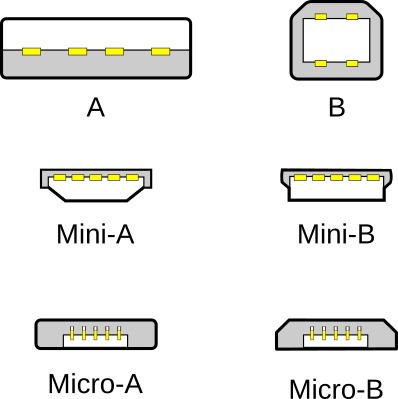
\includegraphics[width=0.28\textwidth]{usbconector}
	\caption{Tipos de conectores USB. Los tipo A deben ser usados en el extremo del Host y los tipo B hacia los periféricos\cite{USBHardwareWiki}}
	\label{fig:con}
\end{figure}

Cada uno de estos dispositivos diferentes, se inteconectan entre sí a través de cables y conductores específicos, diseñados en forma tal que no sea posible conectarlos en forma equivocada. Para cumplir con la norma, el Host debe tener siempre un zócalo compatible con conectores tipo A y los periféricos para enchufes de tipo B. Se observan las diferencias entre uno y otro en la Figura \ref{fig:con}. Los cables de conexión poseen dos pares de conductores: uno para la señal de alimentación de \SI{5}{\volt} ($V_{BUS}$ y $GND$) y otro para el flujo de datos ($D+$ y $D-$).\\

%TODO velociades (interconexión eléctrica)
A nivel eléctrico, la interconexión de datos en los dispositivos se lleva a cabo a través de una codificación de inversión sin retorno a cero, es decir, el cambio de nivel de tensión representa un '0' y el no cambio representa un '1'. Además, la señal de datos es diferencial. Esto implica que cuando $D+$ es positivo, $D-$ debe ser negativo y viceversa.\\

Cabe destacar que, al tener una señal diferencial, la norma USB es {half-dulpex \it}, es decir, puede transmitir en los dos sentidos (desde Host hacia Funciones y viceversa), pero no puede hacerlo en simultáneo\cite{Riihonen2015}, sino que primero debe transmitir un dispositivo y, al finalizar este, el otro es el que tiene acceso al bus.\\

La velocidad de conmutación en los niveles de tensión de la señal de comunicación puede darse a diferentes valores, dando lugar a tres tipos de tasa de bit: Alta-velocidad ({\it High-Speed}) implica una tasa de bit de \SI{480}{\mega\bit\per\second}, Velocidad-completa ({\it Full-Speed}) posee una tasa de bit de \SI{12}{\mega\bit\per\second} y baja-velocidad ({\it Low-Speed}) transmite a una tasa de bit de \SI{1.5}{\mega\bit\per\second}.\\

%TODO revisar lo siguiente(paquetes)
Cuando el Host se comunica con las diferentes Funciones, lo realiza a través de paquetes. Los paquetes implican que la información que se transmite a través del bus está encapsulada en un formato establecido. Cada vez que un dispositivo accede al bus, lo debe hacer de una manera particular definido por el tipo de transferencia, por su rol (Host, Hub o Función) y por el estado de la transmisión dentro del protocolo establecido.